\documentclass{HM}
\newcommand\course{HM 2}
\newcommand\hwnumber{Präsenz 1}   

\usepackage{pgfplots}
\pgfplotsset{compat = newest}

\begin{document}
	\begin{enumerate}
		\item[1.1] Berechne das Taylor-Polynom von $f=\exp$ vom Grad 3 um den Entwicklungspunkt $a=2$
		 $$\text{Taylor-Polynom: }\sum\limits_{n=0}^g\frac{f^{(n)}(a)}{n!}(x-a)^n$$
		 \begin{align*}
		 	\Rightarrow g=3, a=2: 
		 	&\sum\limits_{n=0}^3\frac{(e^2)^{(n)}}{n!}(x-2)^n\\
		 	=&e^2\sum\limits_{n=0}^3\frac{(x-2)^n}{n!}\\
		 	=&\frac{1}{6}e^2(x-2)^3+\frac{1}{2}e^2(x-2)^2+e^2(x-2)^1+e^2
		 \end{align*}
		 
		 \item[1.2] Eine Rakete soll ins Weltall fliegen! Hat die Rakete eine Ruhemasse $m_0$ und Geschwindigkeit $v$, so ist ihre \textit{relativistische Energie} gegeben durch
		 $$E_{rel}=\frac{m_0c^2}{\sqrt{1-(\frac{v}{c})^2}},$$
		 wobei $c$ die Lichtgeschwindigkeit im Vakuum ist. Mit $f: (-\infty,1)\to\R, f(x)\coloneqq\frac{1}{\sqrt{1-x}}$ gilt $E_{rel}=m_0c^2f((\frac{v}{c})^2)$.
		 \begin{enumerate}
		 	\item Berechne das Taylor-Polynom von $f$ vom Grad 1 um den Entwicklungspunkt $a=0$. Welche Näherung für $E_{rel}$ erhält man daraus? Gib die physikalische Interpretation der auftretenden Terme an.
		 	$$\text{Taylor-Polynom: }\sum\limits_{n=0}^g\frac{f^{(n)}(a)}{n!}(x-a)^n$$
		 	\begin{align*}
		 		\Rightarrow g=1, a=0:
		 		&\sum\limits_{n=0}^1\frac{f^{(n)}(0)}{n!}x^n\\
		 		=&\frac{1}{\sqrt{1-0}}+\frac{d}{da}\left(\frac{1}{\sqrt{1-a}}\right)x\\
		 		=&1+\frac{-\frac{d}{da}\sqrt{1-a}}{1-0}x\\
		 		=&1-\frac{1}{2}(1-0)^{-\frac{1}{2}}\frac{d}{da}(1-a)x\\
		 		t_2(x)=&1+\frac{1}{2}x
			\end{align*}
			$\Rightarrow E_{rel}\approx m_0c^2(1+\frac{1}{2}(\frac{v}{c})^2) \Rightarrow E_{rel0}\xrightarrow{v\to c}\frac{3}{2}E_{rel0}$
			$\Rightarrow$ Die maximale \textit{relativistische Energie} beträgt in dieser Näherung 150\% der Ruheenergie.
		 	
		 	\item Gib das Lagrange'sche Restglied $R_1(x)$ für den Entwicklungspunkt $a=0$ an. Wie gut ist die Näherung aus Teil (a) im Fall $m_0=15000kg$ und $v=11\frac{km}{s}$?
		 	$$\text{Lagrange-Restglied: }R_g(x)=f(x)-t_2(x)=\frac{1}{\sqrt{1-x}}-1-\frac{1}{2}x$$
		 	Für $v=11\frac{km}{s}\Rightarrow E_{rel0}\approx 1.3451\cdot 10^{21}, E_{rel1}\approx 1.3481\cdot 10^{21}\Rightarrow E_{rel0}\cdot 1.0022\approx E_{rel1}$\\
		 	$\Rightarrow$ Der Fehler ist $<2.3\%$\\
		 	$\Rightarrow$ Eine gute Näherung für diese Werte\\
		 	
%		 	$$\text{Lagrange-Restglied: }R_g(x)=\frac{f^{(g+1)}(\xi)}{(g+1)!}(x-a)^{g+1}$$
%		 	\begin{align*}
%		 		\Rightarrow g=1, a=0:
%		 		&\frac{f^{(2)}(\xi)}{2!}x^2; \xi\in(-\infty,1]\\
%		 		=&\frac{\frac{d}{dx}\frac{-\frac{1}{2}(1-\xi)^{-\frac{1}{2}}}{1-\xi}}{2}x^2\\
%		 		=&\frac{\frac{d}{dx}-\frac{(1-\xi)^{-\frac{1}{2}}}{2(1-\xi)}}{2}x^2\\
%		 		=&\frac{\frac{d}{dx}-\frac{1}{2(1-\xi)^{\frac{3}{2}}}}{2}x^2\\
%		 		=&\frac{\frac{\frac{d}{dx}2(1-\xi)^{\frac{3}{2}}}{4(1-\xi)^{\frac{6}{2}}}}{2}x^2\\
%		 		=&\frac{\frac{3(1-\xi)^{\frac{1}{2}}}{4(1-\xi)^{\frac{6}{2}}}}{2}x^2\\
%		 		\Rightarrow R_1(x)=&\frac{3}{8(1-\xi)^{\frac{5}{2}}}x^2\\
%		 	\end{align*}
		 	
		 \end{enumerate}
		 
		 \item[1.3] Für $x\in\R$ sei $\floor{x}$ die eindeutig bestimmte Zahl $m$ mit $m\leq x < m+1$. Sind die folgenden Funktionen $\varphi_1,\varphi_2:[0,2]\to\R$ Treppenfunktionen? Wenn ja, bestimme das Integral.
		 \begin{enumerate}
		 	\item $\varphi_1(x)=\sin x$\\
		 	$\varphi_{1_1}:[0,\frac{\pi}{2}]\to[0,1]$ bijektiv und $\varphi_{1_2}:[\frac{\pi}{2},2]\to[\sin2,1]$ bijektiv.\\
		 	Bijektivität widerspricht einer Treppenfunktion, da diese den selben Funktionswert in einem bestimmten Funktionswert aufweist.\\
		 	$\Rightarrow \varphi_1\not\in T$
		 	
		 	\newpage
		 	\item $\varphi_2(x)=\floor{x^2}$
		 	\begin{align*}
		 	a_n\coloneqq&(\sqrt{n}) \text{ mit } n\in\N_0\\ 
		 	\varphi_2(x)=&\begin{cases}
		 	0&0\leq x<1\\
		 	1&1\leq x<\sqrt{2}\\
		 	2&\sqrt{2}\leq x<\sqrt{3}\\
		 	3&\sqrt{3}\leq x<2\\
		 	\hdots&\hdots\\
		 	n&a_n\leq x<a_{n+1}
		 	\end{cases}
		 	\end{align*}
		 	$\Rightarrow \varphi_2\in T$
		 	$$\int_0^b\varphi_2(x)dx=\left(\sum\limits_{k=1}^{\floor{b^2}}(a_{k}-a_{k-1})\varphi_2(a_{k-1})\right)+(b^2-\floor{b^2})\varphi_2(b^2)$$
		 	\begin{align*}
		 	\Rightarrow &\int_0^2\varphi_2(x)dx\\
		 	=&\sum\limits_{k=1}^{4}(\sqrt{k}-\sqrt{k-1})\floor{\sqrt{k-1}^2}+0\\
		 	=&\sum\limits_{k=1}^{4}(\sqrt{k}-\sqrt{k-1})(k-1)\\
		 	=&0+(\sqrt{2}-1)+2(\sqrt{3}-\sqrt{2})+3(2-\sqrt{3})\\
		 	=&-1-\sqrt{2}-\sqrt{3}+6\\
		 	\approx&1.8537
		 	\end{align*}
		 \end{enumerate}
		 
		 \newpage
		 \item[1.4] Sei $f:[0,1]\to\R, f(x)\coloneqq x^2$. Sei $n\in\N$ und betrachte die Zerlegung $0=x_0<x_1<\hdots<x_n=1$ von $[0,1]$, wobei $x_k\coloneqq\frac{k}{n}$. Betrachte Treppenfunktionen $\varphi_n,\psi_n$ mit $\varphi_n\leq f\leq\psi_n$ und
		 $$\varphi_n(x)=\inf\limits_{x_{k-1}<t<x_k}f(t),\quad \psi_n(x)=\sup\limits_{x_{k-1}<t<x_k}f(t)$$
		 für alle $x\in(x_{k-1}, x_k)$.
		 \begin{enumerate}
		 	\item Skizziere $\varphi_3$ und $\psi_3$.\\
		 	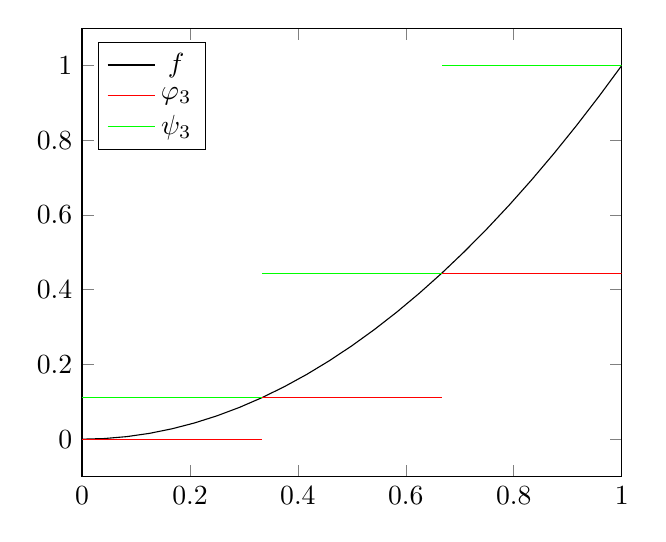
\begin{tikzpicture}
    				\begin{axis}[xmin=-0, xmax=1, ymin=-0.1, ymax=1.1, legend pos = north west]
       				\addplot[domain=0:1] {x^2};
       				\addplot[domain=0:1/3, red] {(0/3)^2};
       				\addplot[domain=0:1/3, green] {(1/3)^2};
       				\addplot[domain=1/3:2/3, red]{(1/3)^2};
       				\addplot[domain=1/3:2/3, green] {(2/3)^2};
       				\addplot[domain=2/3:1, red]{(2/3)^2};
       				\addplot[domain=2/3:1, green] {1};
       				\legend{
    						$f$, 
    						$\varphi_3$,
    						$\psi_3$
    					}
    				\end{axis}
			\end{tikzpicture}
		 	\item Berechne $\int_0^1\varphi_n(x)dx$ und $\int_0^1\psi_n(x)dx$.
		 	$$\int_0^1\varphi_n(x)dx=\sum\limits_{k=1}^n(x_k-x_{k-1})f(x_{k-1})=\sum\limits_{k=1}^n(\frac{k}{n}-\frac{k-1}{n})\left(\frac{k-1}{n}\right)^2=\frac{1}{n^3}\sum\limits_{k=0}^{n-1}k^2$$
		 	$$\int_0^1\psi_n(x)dx=\sum\limits_{k=1}^n(x_k-x_{k-1})f(x_{k})=\sum\limits_{k=1}^n(\frac{k}{n}-\frac{k-1}{n})\left(\frac{k}{n}\right)^2=\frac{1}{n^3}\sum\limits_{k=1}^nk^2$$
		 	\newpage
		 	\item Benutze Teil (b), um zu zeigen, dass $f$ Riemann-integrierbar ist und um $\int_0^1f(x)dx$ zu bestimmen.
		 	$$\int_0^1\varphi_n(x)dx=\frac{1}{n^3}\sum\limits_{k=0}^{n-1}k^2=\frac{1}{n^3}\sum\limits_{k=1}^{n-1}k^2$$
		 	$$\lim\limits_{n\to\infty}\int_0^1\varphi_n(x)dx=\lim\limits_{n\to\infty}\frac{1}{n^3}\sum\limits_{k=1}^{n-1}k^2=\lim\limits_{n\to\infty}\frac{1}{n^3}\sum\limits_{k=1}^{n}k^2=\lim\limits_{n\to\infty}\int_0^1\psi_n(x)dx$$
		 	$\Rightarrow \lim\limits_{n\to\infty}\int_0^1\varphi_n(x)dx=\lim\limits_{n\to\infty}\int_0^1\psi_n(x)dx=\int_0^1f(x)dx$\\
		 	$\Rightarrow$ Riemann-integrierbar
		 	\begin{align*}
		 	&\lim\limits_{n\to\infty}\frac{1}{n^3}\sum\limits_{k=1}^{n}k^2\\
		 	=&\lim\limits_{n\to\infty}\frac{n(n+1)(2n+1)}{6n^3}\\
		 	=&\frac{1}{6}\lim\limits_{n\to\infty}\frac{(2n+1)+2(n+1)}{2n}\\
		 	=&\frac{1}{12}\lim\limits_{n\to\infty}\frac{4n+3}{n}\\
		 	=&\frac{1}{12}\lim\limits_{n\to\infty}4+\frac{3}{n}\\
		 	=&\frac{4}{12}\\
		 	=&\frac{1}{3}
		 	\end{align*}
		 	$\Rightarrow \int_0^1f(x)dx=\frac{1}{3}$
		 \end{enumerate}
	\end{enumerate}
\end{document}